\chapter{Backend design}

\section*{Introduction}

\lettrine[lines=2]{T}\\he iwi has a considerable collection of books dedicated to Māori history, which require different versions for different age groups. To organize the content, we will adopt two main approaches. The primary approach will involve organizing the content around critical historical events and figures to provide readers with a comprehensive understanding of Māori history. The secondary approach will align the content with the local primary and secondary school curriculum to make it relevant to the education of younger readers. By adopting these two approaches, we hope to make the library's books accessible and engaging for readers of all ages and backgrounds.

It is recognized that collecting all the necessary images, sounds, or texts for these books can present a considerable challenge. To address this challenge, AI tools will be incorporated at specific decorative points in the book designs to significantly reduce the manual collection work. However, given the current limitations of AI tools, users must be reminded to ensure that appropriate materials are used in critical areas. Guidelines on using the AI tools effectively will be provided, and materials will be reviewed and updated regularly to ensure their accuracy and relevance.

\section{Two structures}

To create a foundation for the ebook design, we have collected significant events in Māori history (Tab~\ref{tab:maori_history}) and assigned them unique identifiers to indicate their respective timelines. 
When generating the ebooks, we must determine the historical stage to which the book belongs, which will enable us to identify the relevant events and ensure that the book's content is correctly contextualized. 
Additionally, we will determine the appropriate grade level for the book, ensuring that the content is suitable for the target audience's age and education level. 
By establishing these parameters, we can create ebooks that are both informative and engaging for readers (Fig~\ref{s-1} and Fig~\ref{s-2}).

\begin{table}[htbp]
  \centering
  \caption{New Zealand Māori History Timeline}
  \label{tab:maori_history}
  \begin{tabular}{|c|L{3cm}|L{5cm}|L{2cm}|}
    \hline
    \textbf{ID} & \textbf{Date Range} & \textbf{Event} & \textbf{Location} \\
    \hline
    1 & c. 800-1300 & Polynesian ancestors arrive in New Zealand and establish settlements & Multiple \\
    \hline
    2 & 1642 & Dutch explorer Abel Tasman encounters Māori in Golden Bay & South Island \\
    \hline
    3 & 1769-70 & British explorer Captain James Cook charts New Zealand and has first contact with Māori & Multiple \\
    \hline
    4 & 1814-1840 & Musket Wars between Māori tribes for control of resources and territory & North Island \\
    \hline
    5 & 1835 & Declaration of Independence of New Zealand by Māori chiefs & North Island \\
    \hline
    6 & 1840 & Treaty of Waitangi signed between Māori chiefs and British Crown, establishing British sovereignty over New Zealand & North Island \\
    \hline
    7 & 1843-47 & New Zealand Wars fought between Māori and British colonizers & North Island \\
    \hline
    8 & 1860-72 & Land Wars fought between Māori and British colonizers & North Island \\
    \hline
    9 & 1893 & Women's suffrage granted in New Zealand, the first country in the world to do so & Multiple \\
    \hline
    10 & 1975 & Treaty of Waitangi Act established to address Māori grievances and provide restitution & North Island \\
    \hline
  \end{tabular}
\end{table}

In Fig~\ref{s-1}, each grade level has a unique directory with the ability to add or remove directories, making the management of the book's structure more flexible. All books will initially belong to a fixed directory.

\begin{figure}[htbp]
  \centerline{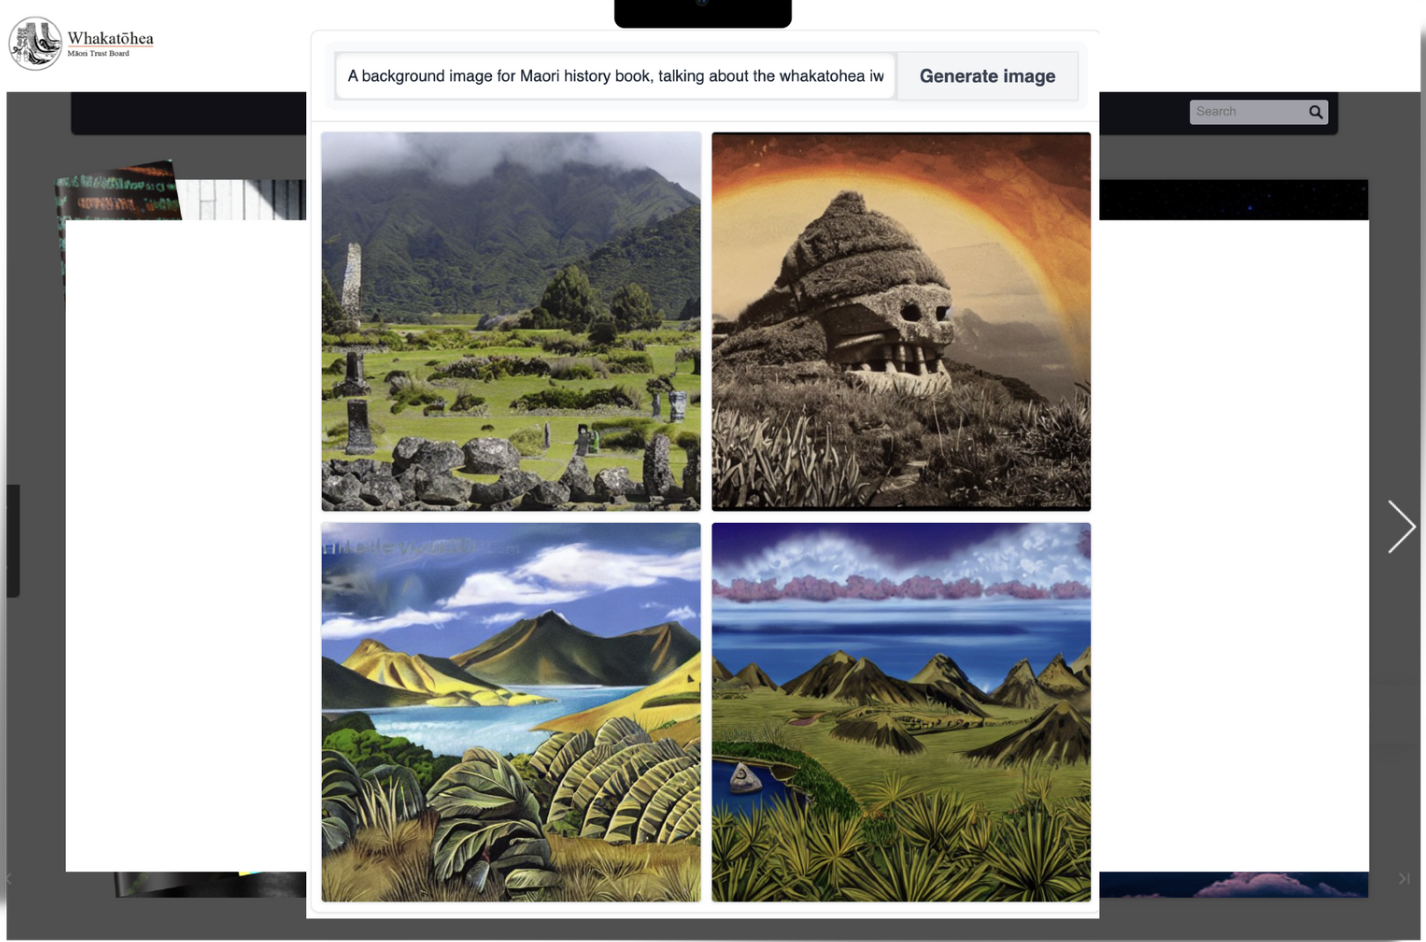
\includegraphics[width=500pt]{images/s-1.png}}
  \caption{Choose different grade levels}
  \label{s-1}
\end{figure}

In Fig~\ref{s-2}, before uploading the necessary materials to generate a book, it is necessary to confirm the historical period to which it belongs. This allows a book under development to potentially belong to both structures simultaneously. This also makes it easier to have a variety of content organization forms in the subsequent prototypes.

\begin{figure}[htbp]
  \centerline{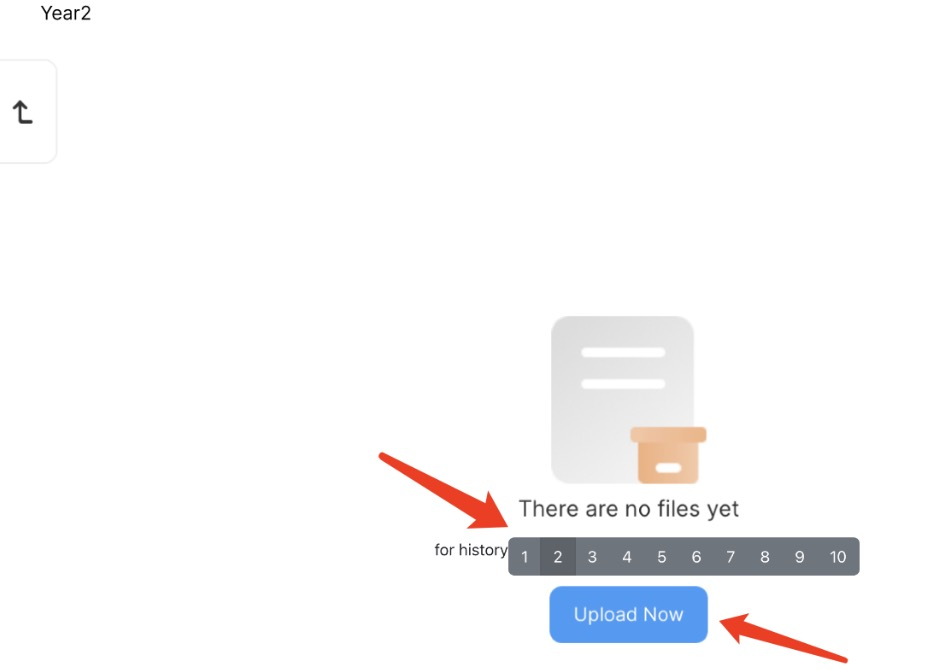
\includegraphics[width=500pt]{images/s-2.jpg}}
  \caption{Choose history and grade levels}
  \label{s-2}
\end{figure}

\section{AI tools}

To reduce the difficulty of finding related materials, non-essential elements such as background images that do not affect the core content but serve a decorative purpose are added in places that are not critical. This enables the book to quickly obtain various styles.

The following functionalities may be required in the backend to improve the convenience of generating books and reduce the need for auxiliary materials:

Built-in image and sound libraries: This would allow for quick access to a collection of images and sounds that are relevant to the book's topic.

Content suggestion engine: This could be an AI-powered tool that suggests related content or sources based on the book's topic.

Integrated translation tools: This would allow for easy translation of the book's content into multiple languages.

Automated formatting and layout tools: This would make it easier to create professional-looking books with consistent formatting and layout.

\section{Conclusion}
Overall, the dual attributes of history and grade curriculum make the organization of books more flexible, and the introduction of AI tools is purely to reduce the difficulty of collecting materials when generating books. 
However, the current AI tools, such as text to image tools, still have high uncertainty in their results and require significant investment. 
This part may be a problem that must be considered, as it is not enough to simply introduce a service provider to complete it.





